

% Set up the document
\documentclass[convert]{standalone}

% Include any extra LaTeX packages required
%\usepackage[square, numbers, comma, sort&compress]{natbib}  % Use the "Natbib" style for the references in the Bibliography

\usepackage{verbatim}  % Needed for the "comment" environment to make LaTeX comments


\usepackage{tabularx,booktabs,adjustbox} % For tables
\usepackage{pdflscape} % For writing some pages in landscape mode
\usepackage{afterpage} % For control over the positioning of figures and tables.

% For pictures
\usepackage{tikz}
\usetikzlibrary{calc,fit,arrows,decorations.pathmorphing,backgrounds,fit,positioning}
\usetikzlibrary{shapes.symbols}

% tikz colour settings
\tikzset{pop1/.style={blue!40},pop2/.style={red!40}}

%% ----------------------------------------------------------------
\begin{document}
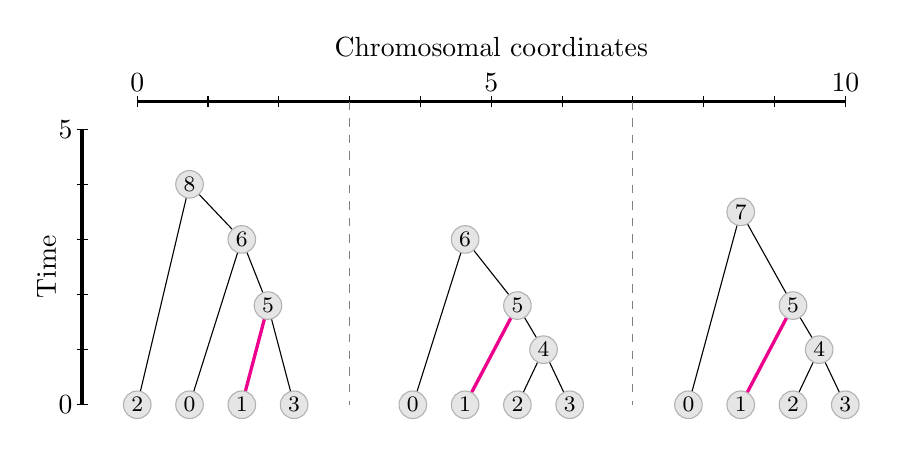
\begin{tikzpicture}[node distance=3mm and 3mm,scale=.7]

\tikzset{greynode/.style={font=\footnotesize,node distance=1cm and 1 cm,fill=black!10,draw=black!30,inner sep=0pt,minimum size=3.5mm,shape=circle},
mutations/.style={shape=starburst,fill=red!50!blue,inner sep=0.8pt,starburst points=11,starburst point height=.2cm}}

% Middle sample nodes
\node (s1) [greynode] {0};
\node (s2) [right=of s1,greynode] {1};
\node (s3) [right=of s2,greynode] {2};
\node (s4) [right=of s3,greynode] {3};

% Left sample nodes
\node (leftTree) at (-5, 0) {};
\node[greynode] (s3l) at ($(s1) + (leftTree)$) {2};
\node[greynode] (s1l) at ($(s2) + (leftTree)$) {0};
\node[greynode] (s2l) at ($(s3) + (leftTree)$) {1};
\node[greynode] (s4l) at ($(s4) + (leftTree)$) {3};

% Right sample nodes
\node (rightTree) at (5, 0) {};
\node [greynode] (s1r) at ($(s1) + (rightTree)$) {0};
\node [greynode] (s2r) at ($(s2) + (rightTree)$) {1};
\node [greynode] (s3r) at ($(s3) + (rightTree)$) {2};
\node [greynode] (s4r) at ($(s4) + (rightTree)$) {3};

% Non-sample nodes
\node [greynode] (s5) at ($0.5*(s3) + 0.5*(s4) + (0,1)$) {4};
\node [greynode] (s5r) at ($(s5) + (rightTree)$) {4};
\node [greynode] (s6) at ($(s3) + (0,1.8)$) {5};
\node [greynode] (s6r) at ($(s6) + (rightTree)$) {5};
\node [greynode] (s6l) at ($0.5*(s2l) + 0.5*(s4l) + (0,1.8)$) {5};
\node [greynode] (s7) at ($(s2) + (0,3)$) {6};
\node [greynode] (s7l) at ($(s2l) + (0,3)$) {6};
\node [greynode] (s8r) at ($(s2r) + (0,3.5)$) {7};
\node [greynode] (s9l) at ($(s1l) + (0,4)$) {8};

% Edges 
\draw[very thick,color=magenta] (s6l) -- (s2l); \draw (s6l) -- (s4l); \draw (s7l) -- (s1l); \draw (s7l) -- (s6l); \draw (s3l) -- (s9l); \draw (s9l) -- (s7l); %tree 1
\draw (s5) -- (s3); \draw (s5) -- (s4); \draw[very thick,color=magenta] (s6) -- (s2); \draw (s6) -- (s5); \draw (s7) -- (s1); \draw (s7) -- (s6); % tree 2
\draw (s5r) -- (s3r); \draw (s5r) -- (s4r); \draw[very thick,color=magenta] (s6r) -- (s2r); \draw (s6r) -- (s5r); \draw (s8r) -- (s1r); \draw (s8r) -- (s6r); % tree 3

% Axes
\node (leftAx) at (-6,0) {};
\draw[very thick] (-6,0) -- +(0, 5);
\foreach \y in {0, 1, 2, 3, 4, 5} \draw ($(leftAx) + (-0.1, \y)$) -- ($(leftAx) + (0.1, \y)$); % tick marks
\draw[very thick] ($(s3l) + (0,5.5)$) -- ($(s4r) + (0,5.5)$);
\node (topAx) at (0,5.5) {};
\node (topLeft) at ($(s3l) + (0,5.5)$) {};
\node (genUnit) at ($0.1*(s4r) - 0.1*(s3l)$) {};
\foreach \x in {0, 1, 2, 3, 4, 5, 6, 7, 8, 9, 10} \draw ($(topLeft) + \x*(genUnit) + (0,0.1)$) -- +(0, -0.2); % tick marks
\node[anchor=east] at ($(leftAx)$) {0}; \node[anchor=east] at ($(leftAx) + (0,5)$) {5};
\node[anchor=south] at ($(topLeft)$) {0}; \node[anchor=south] at ($(topLeft) + 5*(genUnit)$) {5}; \node[anchor=south] at ($(topLeft) + 10*(genUnit)$) {10};

% Interval endpoints
\draw[thin,color=black!50,dashed] ($(topLeft) + 3*(genUnit)$) -- +(0, -5.5);
\draw[thin,color=black!50,dashed] ($(topLeft) + 7*(genUnit)$) -- +(0, -5.5);

% Axis titles
\node (topLabel) at ($(topLeft) + 5*(genUnit) + (0,1)$) {$\textrm{Chromosomal coordinates}$};
\node[rotate=90,anchor=south] (leftLabel) at ($(leftAx) + (-0.3,2.5)$) {$\textrm{Time}$};

\end{tikzpicture}
\end{document}  % The End
%% ----------------------------------------------------------------